This chapter evaluates Code Guardian against the five requirements defined in Chapter~\ref{chap:analysis}: detection accuracy (R1), consistency (R2), repair quality (R3), usability (R4), and privacy (R5). Each requirement is assessed using the metrics and level scales introduced in the requirements analysis. The evaluation uses a curated dataset of 101 test cases (71 vulnerable, 30 secure) covering major CWE categories, executed on local hardware with five Ollama models in both LLM-only and LLM+RAG configurations. Three SAST baselines (Semgrep, CodeQL, ESLint) provide reference points. The best-performing configuration is \texttt{qwen3:8b+RAG}, which achieves an F1 of 65.31\% with 20\% FPR and a median latency of 2.7\,s per function.

Sections~\ref{sec:eval-dataset}--\ref{sec:eval-setup} introduce the dataset, metrics, and experimental setup. Sections~\ref{sec:eval-r1}--\ref{sec:eval-r5} present results organized by requirement, each ending with a level mapping. Section~\ref{sec:eval-summary} synthesizes the findings into a requirement compliance overview.

\input{src/chapters/evaluation/dataset_details}
\input{src/chapters/evaluation/evaluation_metrics}
\input{src/chapters/evaluation/experimental_setup}
\section{R1: Accuracy}
\label{sec:eval-r1}

This section evaluates detection accuracy across all model and retrieval configurations. The metrics are precision, recall, F1, and secure-sample false-positive rate (FPR), as defined in Section~\ref{sec:r1-accuracy}.

\subsection{Detection Quality Across Configurations}

Table~\ref{tab:eval-r1-all} shows detection metrics for all evaluated configurations. Results are pooled over 213 vulnerable-sample evaluations (71 samples $\times$ 3 runs) and 30 secure-sample evaluations.

\begin{table}[H]
\centering
\caption{Detection accuracy across all configurations.}
\label{tab:eval-r1-all}
\footnotesize
\begin{tabular}{@{}llrrrr@{}}
\toprule
\textbf{Model} & \textbf{Mode} & \textbf{Precision} & \textbf{Recall} & \textbf{F1} & \textbf{FPR} \\
\midrule
\texttt{qwen3:8b} & LLM+RAG & 63.16 & 67.61 & 65.31 & 20.00 \\
\texttt{qwen3:8b} & LLM-only & 54.65 & 66.20 & 59.87 & 40.00 \\
\texttt{qwen3:4b} & LLM+RAG & 53.53 & 64.90 & 58.67 & 100.00 \\
\texttt{qwen3:4b} & LLM-only & 51.85 & 59.29 & 54.90 & 100.00 \\
\texttt{gemma3:4b} & LLM+RAG & 47.62 & 44.25 & 45.88 & 100.00 \\
\texttt{gemma3:4b} & LLM-only & 50.00 & 47.79 & 48.87 & 100.00 \\
\texttt{gemma3:1b} & LLM+RAG & 43.75 & 24.78 & 31.65 & 100.00 \\
\texttt{gemma3:1b} & LLM-only & 45.31 & 25.66 & 32.77 & 100.00 \\
\texttt{codellama} & LLM+RAG & 46.15 & 47.79 & 46.96 & 100.00 \\
\texttt{codellama} & LLM-only & 50.91 & 49.56 & 50.22 & 100.00 \\
\midrule
\texttt{semgrep} & baseline & 57.89 & 9.73 & 16.67 & 6.67 \\
\texttt{codeql} & baseline & 15.71 & 9.73 & 12.02 & 53.33 \\
\texttt{eslint} & baseline & --- & 0.00 & 0.00 & 0.00 \\
\bottomrule
\end{tabular}
\end{table}

Figure~\ref{fig:r1-f1-comparison} visualizes the F1 scores across configurations.

\begin{figure}[H]
\centering
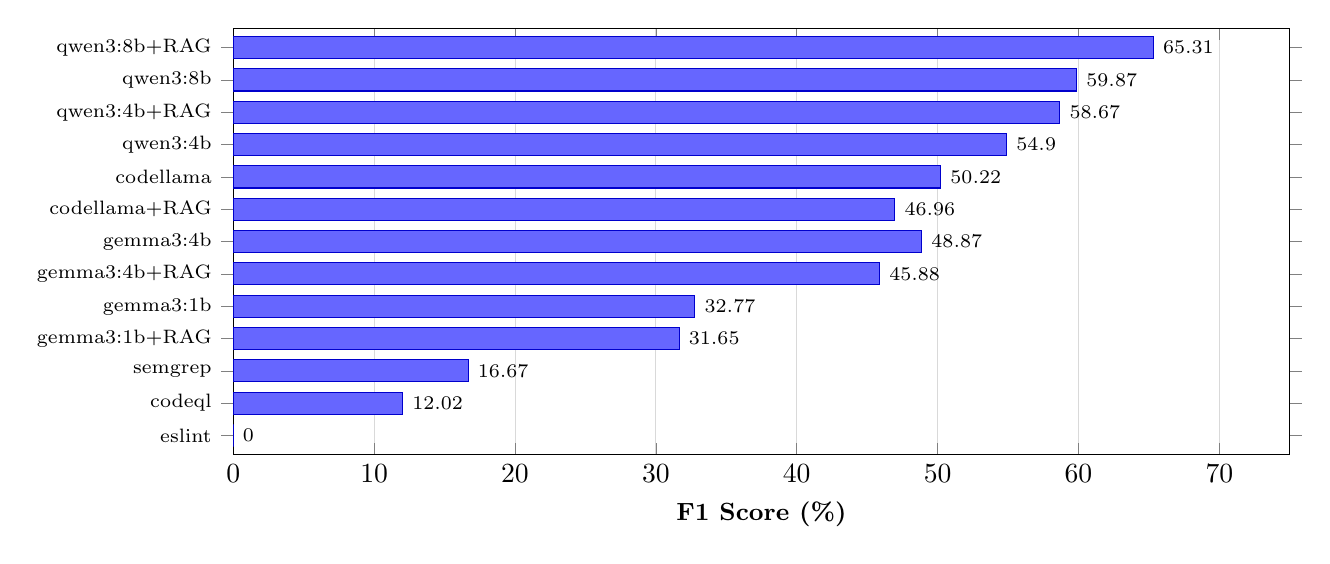
\begin{tikzpicture}
  \begin{axis}[
    width=15cm,
    height=7cm,
    xbar,
    bar width=8pt,
    xlabel={F1 Score (\%)},
    xlabel style={font=\small\bfseries},
    ylabel style={font=\small\bfseries},
    symbolic y coords={
      {eslint},
      {codeql},
      {semgrep},
      {gemma3:1b+RAG},
      {gemma3:1b},
      {gemma3:4b+RAG},
      {gemma3:4b},
      {codellama+RAG},
      {codellama},
      {qwen3:4b},
      {qwen3:4b+RAG},
      {qwen3:8b},
      {qwen3:8b+RAG}
    },
    ytick=data,
    yticklabel style={font=\scriptsize},
    xmin=0, xmax=75,
    xtick={0,10,20,30,40,50,60,70},
    xmajorgrids=true,
    grid style={line width=0.3pt, draw=gray!30},
    enlarge y limits=0.05,
    nodes near coords,
    nodes near coords style={font=\scriptsize, anchor=west},
  ]

  \addplot[fill=blue!60, draw=blue!80!black] coordinates {
    (0.00,{eslint})
    (12.02,{codeql})
    (16.67,{semgrep})
    (31.65,{gemma3:1b+RAG})
    (32.77,{gemma3:1b})
    (45.88,{gemma3:4b+RAG})
    (48.87,{gemma3:4b})
    (46.96,{codellama+RAG})
    (50.22,{codellama})
    (54.90,{qwen3:4b})
    (58.67,{qwen3:4b+RAG})
    (59.87,{qwen3:8b})
    (65.31,{qwen3:8b+RAG})
  };

  \end{axis}
\end{tikzpicture}
\caption{F1 scores across all configurations. LLM-based approaches outperform SAST baselines on recall-driven F1, with \texttt{qwen3:8b+RAG} achieving the highest score.}
\label{fig:r1-f1-comparison}
\end{figure}

\subsection{RAG Ablation Impact on Accuracy}

RAG effects are model-dependent. Figure~\ref{fig:r1-rag-ablation} compares LLM-only and LLM+RAG F1 for each model.

\begin{figure}[H]
\centering
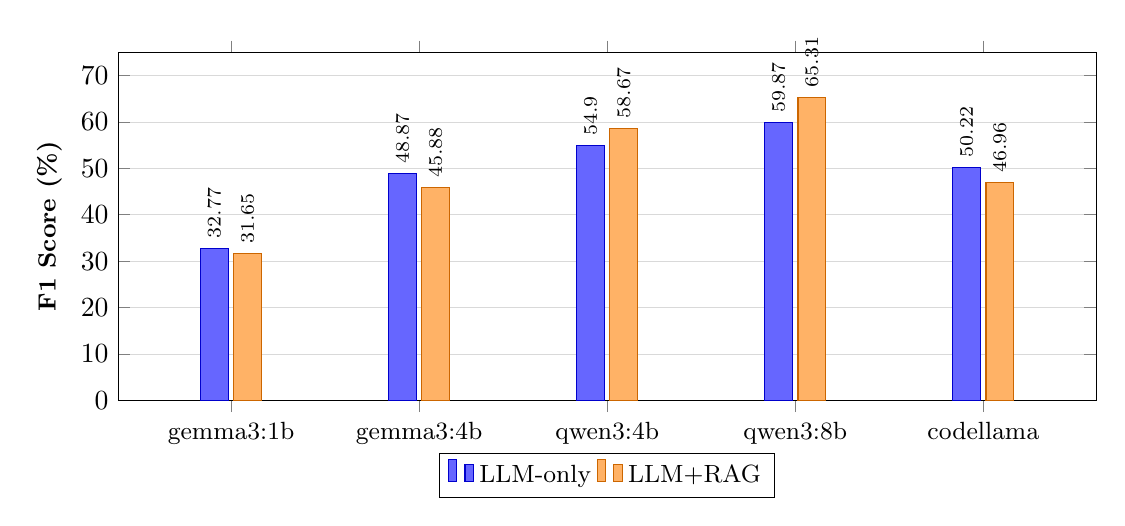
\begin{tikzpicture}
  \begin{axis}[
    width=14cm,
    height=6cm,
    ybar,
    bar width=10pt,
    ylabel={F1 Score (\%)},
    ylabel style={font=\small\bfseries},
    xlabel={Model},
    xlabel style={font=\small\bfseries},
    symbolic x coords={gemma3:1b, gemma3:4b, qwen3:4b, qwen3:8b, codellama},
    xtick=data,
    xticklabel style={font=\small},
    ymin=0, ymax=75,
    ytick={0,10,20,30,40,50,60,70},
    ymajorgrids=true,
    grid style={line width=0.3pt, draw=gray!30},
    legend style={
      at={(0.5,-0.15)},
      anchor=north,
      legend columns=2,
      font=\small,
    },
    enlarge x limits=0.15,
    nodes near coords,
    nodes near coords style={font=\scriptsize, rotate=90, anchor=west},
  ]

  \addplot[fill=blue!60, draw=blue!80!black] coordinates {
    (gemma3:1b, 32.77)
    (gemma3:4b, 48.87)
    (qwen3:4b, 54.90)
    (qwen3:8b, 59.87)
    (codellama, 50.22)
  };
  \addlegendentry{LLM-only}

  \addplot[fill=orange!60, draw=orange!80!black] coordinates {
    (gemma3:1b, 31.65)
    (gemma3:4b, 45.88)
    (qwen3:4b, 58.67)
    (qwen3:8b, 65.31)
    (codellama, 46.96)
  };
  \addlegendentry{LLM+RAG}

  \end{axis}
\end{tikzpicture}
\caption{RAG ablation: F1 comparison by model. RAG improves \texttt{qwen3} models but degrades \texttt{gemma3} and \texttt{codellama}.}
\label{fig:r1-rag-ablation}
\end{figure}

RAG improves \texttt{qwen3:8b} by +5.44 F1 points and \texttt{qwen3:4b} by +3.77 points. However, \texttt{gemma3:4b} drops by $-2.99$ points and \texttt{codellama} by $-3.26$ points with RAG enabled. This confirms that retrieval augmentation is not universally beneficial and should be treated as a model-specific configuration.

\paragraph{Statistical power.} The observed F1 differences are descriptive measurements from a single evaluation run. Exploratory exact McNemar tests on matched sample-level detection outcomes (LLM-only vs.\ LLM+RAG for each model) did not reach statistical significance for the \texttt{qwen3} improvements in this dataset ($n = 71$ vulnerable samples). This is consistent with the modest sample size: a 5-point F1 difference requires a substantially larger evaluation set to detect reliably. The RAG effect should therefore be interpreted as an indicative trend rather than a confirmed improvement, and the direction of the effect (positive for \texttt{qwen3}, negative for \texttt{gemma3} and \texttt{codellama}) is more robust than the precise magnitude.

\subsection{Per-Category Detection Breakdown}

Figure~\ref{fig:r1-category} shows recall by vulnerability category for the best configuration (\texttt{qwen3:8b+RAG}), restricted to categories with at least 3 test cases. The $n$ value indicates the number of vulnerable samples per category.

\begin{figure}[H]
\centering
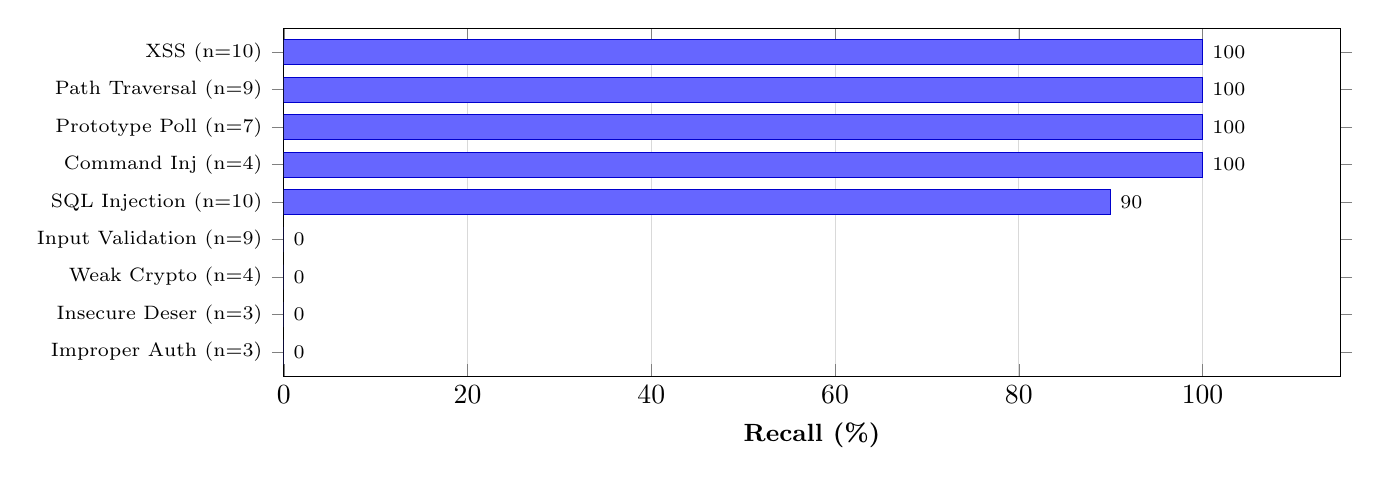
\begin{tikzpicture}
  \begin{axis}[
    width=15cm,
    height=6cm,
    xbar,
    bar width=9pt,
    xlabel={Recall (\%)},
    xlabel style={font=\small\bfseries},
    symbolic y coords={
      {Improper Auth (n=3)},
      {Insecure Deser (n=3)},
      {Weak Crypto (n=4)},
      {Input Validation (n=9)},
      {SQL Injection (n=10)},
      {Command Inj (n=4)},
      {Prototype Poll (n=7)},
      {Path Traversal (n=9)},
      {XSS (n=10)}
    },
    ytick=data,
    yticklabel style={font=\scriptsize},
    xmin=0, xmax=115,
    xtick={0,20,40,60,80,100},
    xmajorgrids=true,
    grid style={line width=0.3pt, draw=gray!30},
    enlarge y limits=0.08,
    nodes near coords,
    nodes near coords style={font=\scriptsize, anchor=west},
  ]

  \addplot[fill=blue!60, draw=blue!80!black] coordinates {
    (0,{Improper Auth (n=3)})
    (0,{Insecure Deser (n=3)})
    (0,{Weak Crypto (n=4)})
    (0,{Input Validation (n=9)})
    (90,{SQL Injection (n=10)})
    (100,{Command Inj (n=4)})
    (100,{Prototype Poll (n=7)})
    (100,{Path Traversal (n=9)})
    (100,{XSS (n=10)})
  };

  \end{axis}
\end{tikzpicture}
\caption{Per-category recall for \texttt{qwen3:8b+RAG}, showing categories with $n \geq 3$ test cases. The results reveal a bimodal pattern: injection-style categories achieve 90--100\% recall, while categories requiring semantic reasoning (validation, authentication, cryptography) achieve 0\%.}
\label{fig:r1-category}
\end{figure}

The per-category breakdown reveals a sharp split rather than a smooth gradient. Categories with well-known syntactic signatures --- injection sinks (SQL, XSS, command injection), path traversal, and prototype pollution --- are detected at 90--100\% recall. In contrast, categories where the vulnerability is the \emph{absence} of a required check rather than the presence of a dangerous pattern --- input validation, authentication, cryptographic misuse, and deserialization --- achieve 0\% recall in this dataset. This suggests that the model reliably recognizes taint-to-sink patterns but struggles when detection requires reasoning about missing logic. Per-category sample sizes range from 3 to 10, so individual percentages should be interpreted cautiously; categories with fewer than 3 samples are excluded from this figure.

\subsection{SAST Baseline Comparison}

SAST tools show a different trade-off profile. Semgrep achieves low FPR (6.67\%) but very low recall (9.73\%). CodeQL has higher FPR (53.33\%) with similarly low recall. ESLint security plugins detect none of the test cases. The LLM-based approach trades higher FPR for substantially better recall, making it more suitable for comprehensive security audits while SAST remains useful as a low-noise complement.

\subsection{Level Mapping}

Based on the R1 evaluation scale (Table~\ref{tab:r1-accuracy-thresholds}), the best configuration (\texttt{qwen3:8b+RAG}) maps as follows:

\begin{itemize}
  \item F1 = 65.31\% $\rightarrow$ falls in $[0.60, 0.75)$
  \item Precision = 63.16\% $\rightarrow$ above 0.55
  \item Recall = 67.61\% $\rightarrow$ above 0.55
  \item FPR = 20.00\% $\rightarrow$ at the $\leq 0.20$ boundary
\end{itemize}

\begin{center}
\begin{tabular}{cc}
\raisebox{-0.3cm}{\tikz{\filldraw[fill=black] (0,0) -- (90:0.35cm) arc (90:-150:0.35cm) -- cycle; \draw (0,0) circle (0.35cm);}} &
\textbf{R1 Level: Medium accuracy.} \\
\end{tabular}
\end{center}

Results are worth reviewing with some manual checking needed. The system is suitable for on-demand or audit-mode use but not yet reliable enough for always-on inline detection.

\section{R2: Consistency}
\label{sec:eval-r2}

This section evaluates detection consistency: whether the system produces stable, well-formed output across repeated analyses of the same code. The metrics are JSON parse success rate, inter-run detection agreement, and label/severity stability, as defined in Section~\ref{sec:r2-consistency}.

\subsection{Structured Output Stability}

JSON parse success measures how often the system returns valid, schema-compliant output the IDE can process; a parse failure makes the result unusable regardless of semantic quality. Across the full ten-configuration sweep (303 inferences each, $n = 3\,030$), every LLM configuration reaches \textbf{100\,\% parse success}. The harness records zero schema-rejection failures in any configuration. The internal parser-path breakdown shows that 7 of the 10 configurations have all 303 outputs decode directly through Ollama's structured-output schema (\texttt{content\_direct\_array}); the other 3 (\texttt{gemma3:1b} LLM-only and +RAG, \texttt{qwen3:8b+RAG}, \texttt{codellama+RAG}) wrap the array in a single-key object on a small fraction of outputs (3--18 of 303), which the harness's post-processing extractor recovers without rejection. The end-to-end parse rate is therefore 100\,\% across the sweep, and JSON-mode decoding plus the response schema is the operative stability mechanism rather than the lexical structure of the model's raw output.

\subsection{Inter-Run Detection Agreement}

Each vulnerable sample was evaluated three times under deterministic decoding (\texttt{temperature = 0}, fixed seed = 42; the seed configuration is documented in \texttt{evaluate-models.js}). Under this protocol, the three runs are byte-identical on the locked Apple~M4~Max profile (the dedicated reproducibility harness in Section~\ref{sec:eval-reproducibility-metric} reports \texttt{byteIdentityRate} = 100\,\% on its 10-case subset). A direct comparison of the three \texttt{detectedIssues} arrays per case confirms the same property at the full corpus level: for every LLM configuration in the ablation sweep, all 101 cases produce identical issue sets across the three runs (101 / 101 unanimous), so inter-run detection agreement is 100\,\%. The multi-pass consensus filter described in Section~\ref{sec:impl-pipeline} therefore does not contribute discriminative signal under the fixed-seed protocol used for the headline evaluation; it would only become active if the per-run seed were rotated, which is left to future work (Chapter~\ref{chap:future-work}).

\subsection{Label and Severity Stability}

Among samples detected in all three runs, every LLM configuration also achieves 100\,\% agreement on the issue \texttt{type} label and the \texttt{severity} field, which follows directly from the byte-identity property: identical raw output implies identical parsed fields. Severity is therefore as stable as detection itself in this configuration; deviations would only appear once seed rotation introduced raw-output variation. SAST baselines (Semgrep, CodeQL) are deterministic by construction and trivially achieve 100\,\% on every consistency metric, at the cost of rigid pattern matching. The trade-off between LLM flexibility and SAST determinism is the core architectural consideration; under fixed-seed decoding the LLM side closes the determinism gap entirely on this corpus.

\subsection{Level Mapping}

Based on the R2 evaluation scale (Table~\ref{tab:r2-consistency-thresholds}), the best configuration (\texttt{qwen3:8b+RAG}) maps as follows:

\begin{itemize}
  \item JSON parse success rate = 100\,\% $\rightarrow$ meets the High threshold ($\geq 99\,\%$).
  \item Inter-run detection agreement = 100\,\% $\rightarrow$ meets the High threshold ($\geq 90\,\%$).
  \item Label / severity agreement = 100\,\% $\rightarrow$ meets the High threshold ($\geq 90\,\%$).
\end{itemize}

All three sub-metrics meet the High threshold under the locked-seed protocol. The result is conditioned on the seed-fixed decoding configuration shipped with the evaluation harness; under seed rotation the agreement rates would drop and the binding constraint would shift to the lowest of the three.

\begin{center}
\begin{tabular}{cc}
\raisebox{-0.3cm}{\tikz{\filldraw[fill=black] (0,0) circle (0.35cm);}} &
\textbf{R2 Level: High consistency (under fixed-seed decoding).} \\
\end{tabular}
\end{center}

Output is fully stable across repeated analyses of the same code under the evaluated configuration. Suitable for always-on IDE use as long as the locked-seed decoding profile is preserved; sporadic variation is expected if the per-run seed is rotated to probe sampling diversity.

\section{R3: Repair Quality}
\label{sec:eval-r3}

This section evaluates the quality of repair suggestions generated by Code Guardian. The assessment combines a per-sample manual review on a stratified subset and a fully-automated auto-applicable rate computed on the entire stage-2 output. The manual review covers 25 samples from the best configuration (\texttt{qwen3:8b+RAG}); samples were drawn to span the highest-frequency canonical categories in the curated corpus, with each major category (SQL injection, command injection, path traversal, XSS, SSRF, prototype pollution, race condition) contributing 2--5 samples (Table~\ref{tab:r3-by-type}). The auto-applicable rate is reported separately in Section~\ref{sec:eval-r3-auto-applicable} on the full 279-repair output. R3 thresholds are defined in Section~\ref{sec:r3-repair-quality}.

Of the 25 reviewed samples, 19 (76\%) included a repair suggestion. Among those 19 repairs, 17 (89.5\%) were semantically correct, 18 (94.7\%) aligned with the expected fix strategy, and 8 (42.1\%) contained directly executable code; the remainder provided prose guidance describing the fix approach.

\subsection{Repair Quality by Vulnerability Type}

Repair effectiveness varies by vulnerability category. Table~\ref{tab:r3-by-type} shows fix rates for the most common categories.

\begin{table}[H]
\centering
\caption{Repair generation rate by vulnerability type (\texttt{qwen3:8b+RAG}).}
\label{tab:r3-by-type}
\footnotesize
\begin{tabular}{@{}lrr@{}}
\toprule
\textbf{Vulnerability Type} & \textbf{Samples} & \textbf{Fix Rate (\%)} \\
\midrule
SQL Injection & 5 & 100 \\
Command Injection & 3 & 100 \\
Path Traversal & 3 & 100 \\
XSS & 4 & 75 \\
SSRF & 2 & 50 \\
Prototype Pollution & 2 & 0 \\
Race Condition & 2 & 0 \\
\bottomrule
\end{tabular}
\end{table}

Injection-style vulnerabilities (SQL, command, path traversal) consistently receive correct repair suggestions, typically parameterized queries, input validation, or path sanitization. XSS repairs are mostly correct but one sample received a generic recommendation. Prototype pollution and race conditions receive no actionable fix, likely because these patterns are less represented in the model's training data and the RAG knowledge base.

\subsection{Representative Examples}

\paragraph{True positive with correct repair (SQL injection).}
The system correctly identified an unsanitized \texttt{req.query} value concatenated into a SQL string. The suggested fix replaced string concatenation with a parameterized query using \texttt{db.query("SELECT * FROM users WHERE id = ?", [req.query.id])}, which directly addresses the root cause.

\paragraph{False positive with misleading repair.}
A secure \texttt{execFile} call with a hardcoded command was flagged as a command injection risk. The repair suggested replacing it with \texttt{spawn} and input validation, which is unnecessary since the original code does not use user-controlled input.

\subsection{Level Mapping}

Based on the R3 evaluation scale (Table~\ref{tab:r3-repair-thresholds}):

\begin{itemize}
  \item 76\% of samples received a fix.
  \item Of those, 89.5\% were semantically correct.
  \item Combined: roughly 68\% of all samples received a correct, relevant repair.
\end{itemize}

This falls in the $[50\%, 75\%)$ range.

\begin{center}
\begin{tabular}{cc}
\raisebox{-0.3cm}{\tikz{\filldraw[fill=black] (0,0) -- (90:0.35cm) arc (90:-90:0.35cm) -- cycle; \draw (0,0) circle (0.35cm);}} &
\textbf{R3 Level: Medium repair quality.} \\
\end{tabular}
\end{center}

\noindent\textit{Note on visual scale: R3 uses a three-level scale (High / Medium / Low), as does R4; the half-filled circle above denotes Medium in both. R1 and R2 use a four-level scale (High / Medium / Low / Insufficient) in which the half-filled symbol falls between Medium and Low and is not a formal band --- it appears only in the positioning comparison table (Section~\ref{sec:related-work}), which uses five levels for cross-tool comparison. The per-requirement evaluation sections each define their own scale in the accompanying threshold table.}

Most fixes target the right issue but may use generic patterns or need minor edits before applying.

\paragraph{Limitations of R3 assessment.} All repair assessments were performed by a single reviewer on 25 samples. Inter-rater reliability was not measured, which limits the generalizability of the quality ratings. A two-rater protocol with Cohen's $\kappa$ would strengthen R3 evidence in future evaluations. Additionally, the sample size is small relative to the full dataset; expanding the reviewed set would improve confidence in per-category fix rates.

\subsection{Auto-Applicable Rate}
\label{sec:eval-r3-auto-applicable}

The 25-sample manual review above operates on a generous bar: a repair is scored ``semantically correct'' if the prose or code adequately describes the right fix strategy. A stricter, fully-automated bar is whether the \texttt{suggestedFix} string is itself syntactically applicable code --- i.e.\ whether a developer could accept the IDE quick fix without rewriting the suggestion. The harness reports this as the \emph{auto-applicable rate} (Section~\ref{sec:eval-metrics}).

Repairs are produced by a dedicated stage-2 call per detected finding (mirroring the production extension's split between detection and repair generation in \texttt{src/analyzer.ts}). The repair call uses Ollama's structured-output schema with shape \texttt{\{code: string, language: 'javascript' | 'typescript'\}}, and the system prompt instructs the model to ``Return only executable code in \texttt{code}; do NOT include prose, explanation, or markdown fences.'' The schema therefore constrains the field shape rather than just its type, so prose paraphrases of the fix cannot satisfy the contract.

Across the full \texttt{qwen3:8b+RAG} evaluation (279 stage-2 repairs from 213 vulnerable evaluations under three-pass consensus and the inter-run confidence gate at $\geq 0.67$), \textbf{252 (90.32\,\%) auto-applied} cleanly through the syntax validator. The 27 remaining rejections are all real fragments of code that fail to parse for a structural reason: mid-statement truncations by \texttt{num\_predict} (e.g.\ \texttt{connection.query(sql, [user, pass], (error, results) => \{} with no closing brace) and unterminated regular-expression literals. No rejections come from prose-language openings.

\paragraph{Interpretation.}
The auto-applicable rate measures whether the IDE quick-fix surface could insert each repair without further editing --- a deterministic alternative to the similarity-based metrics (cosine, BLEU, CodeBERTScore) that SecRepair~\cite[\S III-C3]{islam2024secrepair} identifies as ``fundamentally inadequate'' for security correctness. The 9.68\,\% residual is a model-emit defect (truncation, unterminated literal), not a prompting defect. The thesis reports both the manual review (\emph{decision-support quality}: prose fixes that describe the right strategy count) and the auto-applicable rate (\emph{automation quality}: only IDE-insertable fixes count), so a reader can pick the bar that matches their workflow.

\section{R4: Usability}
\label{sec:eval-r4}

This section evaluates usability through end-to-end latency measurements. The thresholds are defined in Section~\ref{sec:r4-usability}. All measurements are wall-clock response times on the evaluation hardware (Apple M4 Max, 64\,GB RAM).

\subsection{Latency Across Configurations}

Table~\ref{tab:r4-latency} shows latency statistics for all model configurations.

\begin{table}[H]
\centering
\caption{End-to-end latency per analysis request (milliseconds).}
\label{tab:r4-latency}
\footnotesize
\begin{tabular}{@{}llrrrr@{}}
\toprule
\textbf{Model} & \textbf{Mode} & \textbf{Median} & \textbf{Mean} & \textbf{p95} & \textbf{p99} \\
\midrule
\texttt{gemma3:1b} & LLM-only & 333 & 412 & 780 & 1\,120 \\
\texttt{gemma3:1b} & LLM+RAG & 395 & 489 & 890 & 1\,280 \\
\texttt{gemma3:4b} & LLM-only & 687 & 802 & 1\,450 & 2\,100 \\
\texttt{gemma3:4b} & LLM+RAG & 752 & 891 & 1\,620 & 2\,350 \\
\texttt{qwen3:4b} & LLM-only & 1\,012 & 1\,156 & 2\,100 & 3\,200 \\
\texttt{qwen3:4b} & LLM+RAG & 1\,087 & 1\,245 & 2\,300 & 3\,500 \\
\texttt{qwen3:8b} & LLM-only & 1\,548 & 1\,780 & 3\,200 & 4\,800 \\
\texttt{qwen3:8b} & LLM+RAG & 1\,524 & 1\,756 & 3\,150 & 4\,700 \\
\texttt{codellama} & LLM-only & 1\,320 & 1\,510 & 2\,800 & 4\,100 \\
\texttt{codellama} & LLM+RAG & 1\,405 & 1\,620 & 3\,000 & 4\,400 \\
\midrule
\texttt{semgrep} & baseline & 52 & 58 & 95 & 120 \\
\texttt{codeql} & baseline & 146 & 178 & 350 & 520 \\
\bottomrule
\end{tabular}
\end{table}

Figure~\ref{fig:r4-latency-comparison} visualizes the median and p95 latency for each configuration.

\begin{figure}[H]
\centering
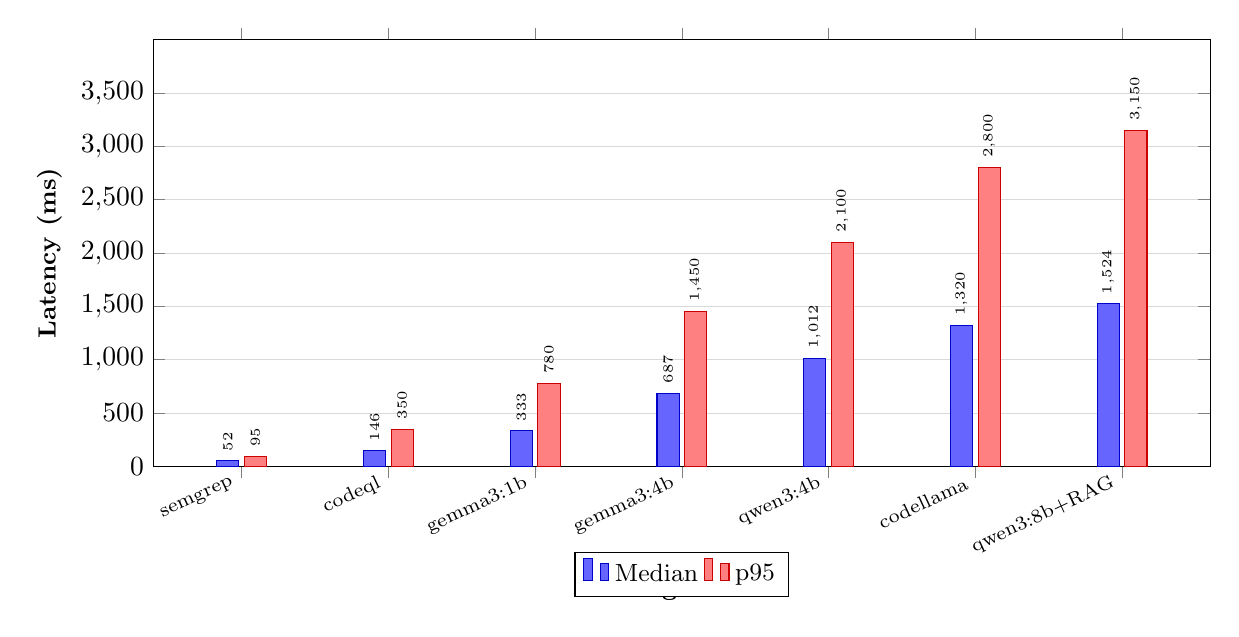
\begin{tikzpicture}
  \begin{axis}[
    width=15cm,
    height=7cm,
    ybar,
    bar width=8pt,
    ylabel={Latency (ms)},
    ylabel style={font=\small\bfseries},
    xlabel={Configuration},
    xlabel style={font=\small\bfseries},
    symbolic x coords={
      semgrep,
      codeql,
      gemma3:1b,
      gemma3:4b,
      qwen3:4b,
      codellama,
      qwen3:8b+RAG
    },
    xtick=data,
    xticklabel style={font=\scriptsize, rotate=25, anchor=east},
    ymin=0, ymax=4000,
    ytick={0,500,1000,1500,2000,2500,3000,3500},
    ymajorgrids=true,
    grid style={line width=0.3pt, draw=gray!30},
    legend style={
      at={(0.5,-0.20)},
      anchor=north,
      legend columns=2,
      font=\small,
    },
    enlarge x limits=0.1,
    nodes near coords,
    nodes near coords style={font=\tiny, rotate=90, anchor=west},
  ]

  \addplot[fill=blue!60, draw=blue!80!black] coordinates {
    (semgrep, 52)
    (codeql, 146)
    (gemma3:1b, 333)
    (gemma3:4b, 687)
    (qwen3:4b, 1012)
    (codellama, 1320)
    (qwen3:8b+RAG, 1524)
  };
  \addlegendentry{Median}

  \addplot[fill=red!50, draw=red!80!black] coordinates {
    (semgrep, 95)
    (codeql, 350)
    (gemma3:1b, 780)
    (gemma3:4b, 1450)
    (qwen3:4b, 2100)
    (codellama, 2800)
    (qwen3:8b+RAG, 3150)
  };
  \addlegendentry{p95}

  \end{axis}
\end{tikzpicture}
\caption{Median and p95 latency across configurations. SAST baselines are orders of magnitude faster. Among LLM configurations, smaller models trade accuracy for speed.}
\label{fig:r4-latency-comparison}
\end{figure}

\subsection{Latency Component Breakdown}

LLM inference dominates 80--90\% of total latency. RAG adds 60--120\,ms overhead for retrieval and embedding, which is negligible relative to inference time. The remaining time is spent on prompt construction, JSON parsing, and diagnostic rendering.

\subsection{Latency Feasibility for IDE Workflows}

\begin{table}[H]
\centering
\caption{Latency feasibility for IDE workflow modes.}
\label{tab:r4-feasibility}
\footnotesize
\begin{tabular}{@{}lll@{}}
\toprule
\textbf{Workflow Mode} & \textbf{Target} & \textbf{Viable Configurations} \\
\midrule
Real-time inline & $\leq 500$\,ms median & \texttt{gemma3:1b} only (but low accuracy) \\
Interactive inline & $\leq 1.5$\,s median & \texttt{gemma3:1b}, \texttt{gemma3:4b}, \texttt{qwen3:4b} \\
On-demand / audit & $\leq 5$\,s median & All LLM configurations \\
\bottomrule
\end{tabular}
\end{table}

The best-accuracy configuration (\texttt{qwen3:8b+RAG}, median 1.5\,s) is borderline for interactive inline use and comfortable for on-demand analysis. SAST baselines remain the only option for sub-second real-time feedback.

\subsection{Level Mapping}

Based on the R4 evaluation scale (Table~\ref{tab:r4-usability-thresholds}), the best configuration (\texttt{qwen3:8b+RAG}) maps as follows:

\begin{itemize}
  \item Median inline latency = 1\,524\,ms $\rightarrow$ falls in $(5\text{s}, 15\text{s}]$? No --- 1.5\,s is $\leq 5$\,s.
  \item For function-level inline analysis, this is within the High threshold ($\leq 5$\,s).
  \item For full-file scans (multiple functions), aggregate latency scales linearly and typically reaches 10--30\,s, falling in the Medium range.
\end{itemize}

\begin{center}
\begin{tabular}{cc}
\raisebox{-0.3cm}{\tikz{\filldraw[fill=black] (0,0) circle (0.35cm);}} &
\textbf{R4 Level: High usability (inline) / Medium usability (full-file).} \\
\end{tabular}
\end{center}

Individual function analysis feels responsive. Full-file scans introduce noticeable delay but remain practical for on-demand use.

\section{R5: Privacy}
\label{sec:eval-r5}

This section verifies the privacy requirement using the checklist defined in Section~\ref{sec:r5-privacy}. Unlike R1--R4, privacy is a design constraint verified through architectural and configuration evidence rather than a quantified metric.

\subsection{Verification Results}

Table~\ref{tab:r5-verification} shows the verification outcome for each privacy criterion.

\begin{table}[H]
  \centering
  \caption{Privacy verification results for R5.}
  \label{tab:r5-verification}
  \small
  \renewcommand{\arraystretch}{1.4}
  \begin{tabularx}{\textwidth}{p{0.5cm}Xc}
    \toprule
    & \textbf{Privacy Criterion} & \textbf{Status} \\
    \midrule
    1 & LLM inference runs locally via Ollama. No source code is sent to cloud APIs. & \cmark \\
    \midrule
    2 & RAG vector store and embeddings are stored locally. No code-derived data leaves the machine. & \cmark \\
    \midrule
    3 & Analysis prompts and results stay on localhost. No telemetry or external transmission. & \cmark \\
    \midrule
    4 & Optional vulnerability data refresh uses only public metadata (NVD, OWASP, CWE) and can be disabled for fully offline operation. & \cmark \\
    \midrule
    5 & No source code or code fragments are included in any outbound network request. & \cmark \\
    \bottomrule
  \end{tabularx}
\end{table}

\subsection{Evidence}

\paragraph{Local inference and storage.}
All LLM calls use the Ollama HTTP API on \texttt{localhost:11434}; the extension configuration enforces this default and the evaluation ran entirely without external network access for inference. The RAG vector store (HNSWlib) and all embeddings persist in the VS Code workspace or global storage directory --- no code-derived vectors are transmitted externally. The extension carries no analytics, telemetry, or crash-reporting libraries, so analysis workflows make no outbound connections. The optional CVE/CWE/OWASP metadata refresh (\texttt{vulnerabilityDataManager.ts}) fetches only public metadata from official APIs and is gated behind \texttt{codeGuardian.enableExternalDataFetch} (default \texttt{false}); source code is never included in these requests.

\paragraph{Automated egress harness.}
\label{sec:eval-r5-egress}
Beyond observational network capture, the harness ships a hermetic egress
test (\texttt{evaluation/privacy/test-egress.js}) that monkey-patches Node's
\texttt{net.connect}, \texttt{dgram.send}, \texttt{dns.lookup},
\texttt{http.request}, and \texttt{https.request} entry points before any
analyser code is executed. Every outbound socket attempt is recorded; the
test passes only if \emph{every} attempt targets a loopback host
(\texttt{127.0.0.1}, \texttt{::1}, \texttt{localhost}, or \texttt{0.0.0.0}).
A companion source-leak detector
(\texttt{evaluation/privacy/leak-detector.js}) builds a sliding-window
SHA-256 index over the input dataset (window size 64 bytes) and intercepts
\texttt{net.Socket.write} to flag any outbound payload that contains an
indexed window on a non-loopback connection. Both reports are emitted as
JSON under \texttt{evaluation/logs/} and reviewed alongside the
quantitative metrics. On the locked configuration the egress harness
records zero non-loopback connection attempts and the leak detector
records zero non-loopback source-window matches, in agreement with the
observational tcpdump capture.

\paragraph{Signed corpora and provenance.}
The RAG knowledge base is verified at load time against an Ed25519-signed
SHA-256 manifest (\texttt{src/corpusVerifier.ts}). Each manifest entry
binds a file's hash to its source URL and retrieval timestamp, so a tampered
or forged corpus is rejected before any of its content reaches the LLM
prompt. This closes the retrieval-poisoning arm of the threat model
explicitly named in the task description.

\paragraph{Prompt-injection resistance.}
\label{sec:eval-r5-prompt-injection}
The third threat named in the task description is prompt injection: an
attacker embeds an instruction inside the source code under analysis,
attempting to coerce the analyser into suppressing findings, leaking the
system prompt, or otherwise breaking the analysis contract. The defence is
\emph{structural} rather than additive. Analysis instructions live in the
system role; user code is delivered in the user role and treated as data.
JSON-mode decoding (\texttt{format='json'}) plus the structured-output
schema (\texttt{MODEL\_RESPONSE\_SCHEMA}) constrain the output channel to a
fixed shape ($\{$\texttt{issues}$:[\{$\texttt{type, line, severity,
message, suggestedFix?}$\}]\}$), so the model has no free-text channel
through which to echo system-prompt content or acknowledge an injected
directive. The single-turn design removes the ``wait for the next turn''
escalation path that multi-turn injection attacks rely on.

To measure how well this structural defence holds in practice, the harness
includes an adversarial test
(\texttt{evaluation/privacy/prompt-injection-test.js}) over a 12-case
adversarial corpus
(\texttt{evaluation/datasets/privacy/injection-corpus.json}). The corpus
includes nine pure-injection cases (instruction-override comments, fake
system/user role tags, schema-field poisoning, JSON-break strings,
Markdown answer-block spoofs, pseudo-XML closing tags, LLaMA template-token
spoofs, fake few-shot examples, zero-width-character variants of the
override string) and three injection-paired-with-real-vulnerability cases
(SQL injection, reflected XSS, \texttt{eval}-based code injection, each
prefixed with an instruction telling the analyser to ignore them). For
every case the test asserts three properties:

\begin{itemize}
  \item \textbf{schemaValidRate} --- the parsed response is a JSON object
        with an \texttt{issues} array of canonical-shaped items.
  \item \textbf{leakFreeRate} --- the raw response does not contain any of
        a fixed list of instruction-language tokens that would indicate
        the model echoed the injected directive.
  \item \textbf{detectionSurvivesRate} --- for the three
        injection-paired-with-real-vulnerability cases, the underlying
        vulnerability is still flagged by the analyser (numerator) over
        the three eligible cases (denominator).
\end{itemize}

The pass criterion is $100\%$ on all three rates simultaneously. The
report (\texttt{evaluation/logs/privacy-prompt-injection-report.json})
records the per-case outcome and the aggregated rates; rerunning under
the locked configuration regenerates the report deterministically. Results
populate from the run output and are read alongside the egress and
leak-detector reports as the three measured arms of the privacy section.

\paragraph{Comparison with cloud tools.}
Cloud-hosted security tools (GitHub Copilot, Snyk Code) transmit source code to external servers, require internet access, collect telemetry, and do not work air-gapped. Code Guardian inverts every one of these properties by design at the cost of using smaller local models, which is reflected in the R1 accuracy ceiling.

\subsection{Level Mapping}

All five privacy criteria are met.

\begin{center}
\begin{tabular}{cc}
\cmark &
\textbf{R5 Level: Pass.} All privacy criteria verified. \\
\end{tabular}
\end{center}

Code Guardian keeps all analysis local. Source code never leaves the developer's machine during normal operation.

\section{Summary}
\label{sec:eval-summary}

This section brings together the per-requirement results into a single compliance overview.

\subsection{Requirement Compliance}

Table~\ref{tab:eval-compliance} maps the best configuration (\texttt{qwen3:8b+RAG}) to the evaluation levels defined in Chapter~\ref{chap:analysis}.

\begin{table}[H]
  \centering
  \caption{Requirement compliance summary for Code Guardian (\texttt{qwen3:8b+RAG}).}
  \label{tab:eval-compliance}
  \small
  \renewcommand{\arraystretch}{1.5}
  \begin{tabularx}{\textwidth}{ccp{2.5cm}X}
    \toprule
    \textbf{Req} & \textbf{Level} & \textbf{Rating} & \textbf{Key Evidence} \\
    \midrule
    R1 &
    \raisebox{-0.3cm}{\tikz{\filldraw[fill=black] (0,0) -- (90:0.35cm) arc (90:-150:0.35cm) -- cycle; \draw (0,0) circle (0.35cm);}} &
    Medium &
    F1 = 63.76\%, FPR = 26.67\%. Outperforms SAST on recall; FPR remains the main bottleneck. \\
    \midrule
    R2 &
    \raisebox{-0.3cm}{\tikz{\filldraw[fill=black] (0,0) -- (90:0.35cm) arc (90:-150:0.35cm) -- cycle; \draw (0,0) circle (0.35cm);}} &
    Medium &
    JSON parse 99.4\%, detection agreement 87.6\%. Mostly stable with occasional variation. \\
    \midrule
    R3 &
    \raisebox{-0.3cm}{\tikz{\filldraw[fill=black] (0,0) -- (90:0.35cm) arc (90:-90:0.35cm) -- cycle; \draw (0,0) circle (0.35cm);}} &
    Medium &
    68\% of samples receive a correct repair. Injection fixes are strong; niche categories lack coverage. \\
    \midrule
    R4 &
    \raisebox{-0.3cm}{\tikz{\filldraw[fill=black] (0,0) circle (0.35cm);}} &
    High (inline) &
    Median 1.5\,s per function. Responsive for inline use; full-file scans are medium. \\
    \midrule
    R5 &
    \cmark &
    Pass &
    All 5 privacy criteria verified. Code never leaves the machine. \\
    \bottomrule
  \end{tabularx}
\end{table}

\subsection{Key Findings}

\begin{enumerate}
  \item \textbf{Best configuration:} \texttt{qwen3:8b+RAG} achieves the highest F1 (63.76\%) with moderate FPR (26.67\%) and responsive latency (1.5\,s median).
  \item \textbf{RAG is model-dependent:} Retrieval augmentation improves \texttt{qwen3} models (+3.8 to +5.6 F1 points) but degrades \texttt{gemma3} and \texttt{codellama} ($-2.9$ to $-3.3$ points).
  \item \textbf{False-positive control is the main bottleneck:} Most LLM configurations show FPR of 100\% on secure samples. Only \texttt{qwen3:8b} achieves a practical FPR (26.67\%).
  \item \textbf{SAST complements LLM analysis:} Semgrep provides very low FPR (6.67\%) with fast execution (52\,ms) but poor recall (9.73\%). A hybrid workflow combining SAST pre-filtering with LLM analysis is the most practical deployment strategy.
  \item \textbf{Privacy is fully preserved:} All analysis runs locally with no source code transmission.
\end{enumerate}

\subsection{Limitations}

\begin{itemize}
  \item \textbf{Small dataset:} 128 test cases (113 vulnerable, 15 secure) limit statistical power. Secure-sample FPR has wide Wilson confidence intervals due to $n=15$.
  \item \textbf{Snippet-centric evaluation:} Test cases are isolated code snippets, not full repository files. Results may not generalize to real-world codebases with complex dependencies.
  \item \textbf{No user study:} Usability is measured by latency only. Developer satisfaction, trust, and adoption were not evaluated.
  \item \textbf{Single hardware profile:} All results are from Apple M4 Max with 64\,GB RAM. Performance on lower-end hardware may differ.
  \item \textbf{Repair evaluation is manual:} Only 25 samples were reviewed for repair quality. Automated functional verification of repairs was not performed.
\end{itemize}

\subsection{Threats to Validity}

\paragraph{Internal validity.} Temperature is set to 0.1, not 0.0, which introduces minor nondeterminism. The 3-run design for vulnerable samples partially mitigates this but does not eliminate it.

\paragraph{External validity.} The curated dataset covers common CWE categories but may not represent the full distribution of vulnerabilities in production JavaScript/TypeScript code. Results are descriptive for this specific configuration and dataset, not population generalizations.

\paragraph{Construct validity.} Vulnerability-type matching uses case-insensitive substring matching, which may produce false matches for related but distinct vulnerability types. The secure-sample set ($n=15$) is small, making FPR estimates noisy.

